\section{Experiments}

\subsection{Training Data}
To train our model we use a subset of the dataset provided by the \gls{stc} as well as the ArchiMob corpus. The \gls{stcd} contains 38 GB (ca. 150k files) of labelled, 65 GB of unlabelled spoken swiss german audio data and an additional validation set
containing 1.5 GB of data \cite{stc2019}. The ArchiMob corpus (Release 2) contains X GB of spoken swiss german data \cite{archimob2016}. We remove all audio files from the \gls{stcd} where the quality of the translation
is rated lower than 0.7 (rating provided by \gls{stc}) which are still around 130k files. Additionally, we also need to remove files larger than 1 MB due to memory limitations (ca. 7k files). All files were converted from flac to wav files and the sample rate was reduced from 48'000 Hz to 16'000 Hz to match the DeepSpeech input requirements.
The German DeepSpeech comes with a script to pre-process the transcriptions. This removes all punctuation, converts numbers to their respective text version, converts the text to lowercase and normalizes some characters. This fits the requirements given by the \gls{stc}.

\subsection{Evaluation metrics}
We evaluate our model through two types of metrics. The BLEU score \cite{Papineni2002BleuAM}, which is required by the \gls{stc} to compare the results. The \gls{stc} specifically requires a corpus
based BLEU score (todo cite stc), which aims at measuring the distance/similarity of the generated text and the provided ground truth. As the German DeepSpeech test script does not include the BLEU score we added it manually. \\~\\Additionally, we keep track of the \gls{wer} for our models, as
this is a common metric for speech recognition systems \cite{Park2008AnEA} which is also included in the German DeepSpeech.

\subsection{Environment}
We train the model on a single NVIDIA GeForce RTX 2070 Laptop GPU (8 GB memory). We perform minimal tuning of our model's hyperparameters following the work of \newcite{Agarwal2020LTLUDEAL}.
.

\subsection{Models}
Following \newcite{pluss2020} we use a DeepSpeech architecture \cite{Hannun2014DeepSS} as our main model for speech-to-text translation. In order to get better results we use a
a pre-trained DeepSpeech model \cite{DeepSpeechGerman090} as the base model for most of our experiments. The first model we trained served as our private baseline. \paragraph{Baseline model} We trained a bare DeepSpeech model with the default hyperparameters
on the labelled \gls{stcd} which achieved a BLEU score of 0.0004 BLEU on the official test set. The baseline model will be revered to as baseline model or model \#0 henceforth.\paragraph{Pre-trained model \#1} In order to improve our baseline model we use a pre-trained
german DeepSpeech model \cite{DeepSpeechGerman090}, which is fine-tuned on the \gls{stcd} dataset with the previously mentioned hyperparameters. The model achieved a BLEU score of
XY on the validation set and XY on the test set.
\paragraph{Additional data model \#2} To further improve our \nth{1} model we added additional data to our fine-tuned model. We added the ArchiMob data and fine-tuned for an additional 75 epochs, with
the same hyperparameters as in model \#1 and achieved the following BLEU scores on the validation and trainig set, XYZ, XYZ2, respectively.
\paragraph{ArchiMob data model \#3} As the \nth{2} model did not achieve the expected results we decided to fine-tune our model on the ArchiMob data, as we expected the data distribution to be closer
to the actual test set. We achieved the following BLEU scores for the validation and test set, XYZ, XYZ2,
respectively.
\paragraph{Augmented data model \#4} In order to produce a more robust model, that can handle different pronunciations and speeds, we added data augmentation to our \nth{3} model. We fine-tuned our
model with the following data augmentations:
\begin{itemize}
    \item warp: ''Applies a non-linear image warp to the spectogram. This is achieved by randomly shiting a grid of equally distribted warp points along time and frequency axis''
    \cite{DeepSpeechAugmentation}
    \item tempo: ''Scales spectrogram on time axis and thus changes playback tempo.'' \cite{DeepSpeechAugmentation}
\end{itemize}

The \gls{stcd} dataset is used for the augmentation fine-tuning on the \nth{3} model. This approach achieved a BLEU score of XY on the validation set and XY on the test set. The model was trained for
10 epochs with a warp probability of 0.1 and a tempo probabily of 0.1. We increased the batch size to 36, as the augmentation process per batch took more time than expected. Due to time limitations we
were not able to continue training the model any further, but the model was still improving and we expect that this approach could produce even better results. The \gls{wer} progression is depicted in the following plot:
\begin{figure}[H]
    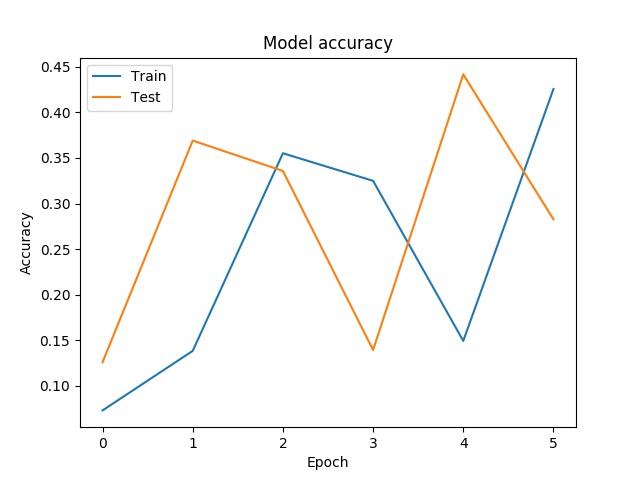
\includegraphics[width=\linewidth,height=5cm]{img/werPlot.png}
    \caption{WER per epoch}
    \label{fig:werPerEpoch}
\end{figure}

\paragraph{Text-to-Text model \#5} Our \nth{5} approach tries to improve the output by adding a text-to-text translation model after the speech-to-text model. We fine tuned a pre-trained german to
english model following \newcite{TiedemannThottingal:EAMT2020} using the ''huggingface'' framework \cite{wolf-etal-2020-transformers} on the \gls{stcd} dataset. With this approach we achieved a BLEU score of XY on the validation dataset and
XY on the test dataset.
